\section{vRNIC Design}
To achieve unified RDMA virtualization, we design vRNICs, which is software virtualization with complete RDMA attributes. Both conatiners and VMs can use vRNICs through unified drivers. 

\subsection{vRNIC Virtualization}
% vRNIC 设计空间探讨

To make vRNIC flexible and hardware-independent, we construt each vRNIC by software methods. Moreover, both kernel-space and user-space are feasible to construct vRNICs in host. Compared to kernel-space, there are multiple advantages for vRNICs in user-space, such as minimal attack surface, flexible management and independent on RDMA kernel drivers. Thus, we choose the user-space for vRNIC virtualization.

We find that RDMA resources (e.g. QP, MR or DoorBells) are the key roles in whole RDMA communication. In control path, the application creates QPs, registers MRs in host memory, map RNIC's doorbell resgisters to host memory and so on; In data path, the application directly use above RDMA resources. For example, application writes DoorBell to notify RNIC to deal with WQE in QP and transport the specific data in MR. Thus, vRNIC virtualization is mainly about how to construct the virtual RDMA resources to provide complete RDMA communication. 

Based on above analysis, we summarize that RNIC has two kinds of hardware properties about these RDMA resources, namely static property and dynamic property:

Static properties are mainly about what RDMA resources are equiped in RNIC. For each RDMA resource, it can be abstracted that RNIC has the corresponding buffers to fillwith dynamic resource instances. For example, each QP is in QP buffer of the vRNIC.

For dynamic attributes, the state of RDMA resources are dynamic in control path and data path. Control path includes the creation and destroy of RDMA resources. RDMA resources instance are changed in RNIC buffer. For example, RNIC records the QP number when QP is created, changes QP state for RDMA connection and clear QP information in the destroy. Note that this process has less latency due to the kernel. Data path is mainly about the usage of RDMA resources. RDMA resources or information in buffer are always maintained in RNIC. When RDMA applications post a send or receive operation, only write the DoorBell and the hardware processor performs DMA, encapsulates and forwards data.

To emulate the static attributes, virtual queue, data and doorbell and unlimited for the numbs of RDMA resources instances. 

\subsection{vRNIC Mapping}
To emulate the dynamic attributes, we need map the vRNIC to physical to realize control path or data path. For example, when application calls post\_send, the vRNICs can drive physical RNIC to transport the corresponding data. Thus, in our design, the vRNIC is flexible for management. 

Fortunately, we found all RDMA resources information in RNIC are only changed in control path and maintained in data path. So, we can map the virtual RDMA resources to RNIC only in control path, such as QP and Doorbell,  and do not need introduce any operations in data path. Mapped RDMA resources are directly used and RNIC is notified by mapped virtual DoorBell in vRNIC. As a result, vRNIC are still with DMA zero-copy, hardware protocol stack processing and other high-performance capability in data path. Therefore, we put each vRNIC with a map unit. As Figure~\ref{fig:map-unit} shows, it maps or unmaps virtual RDMA resources from vRNIC to RNIC in control path:-


\begin{figure}[!ht]
	\centering
	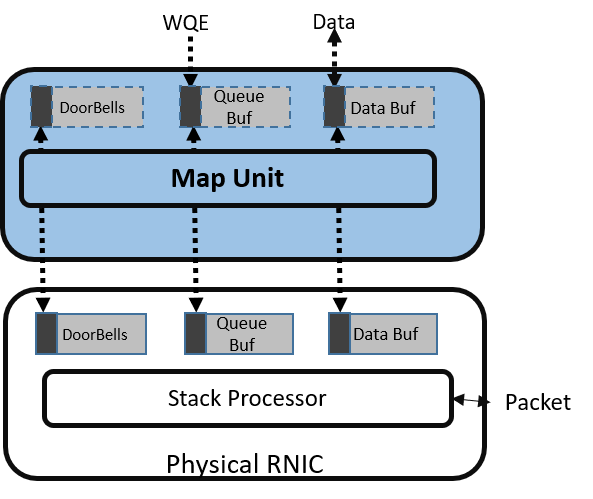
\includegraphics[width=0.9\linewidth]{images/map-unit}
	\caption{Map Unit in vRNIC}
	\label{fig:map-unit}
\end{figure}

For RDMA resources (e.g. QPs, CQs): Taking QP as an example, regularly, vRNIC record virtual RDMA resources information when the virtual QP instance are created. However, virtual QP are still not generated-associated with the RNIC. To make the mapping, the map unit will create corresponding real QP instance in RNIC based on the information of virtual QP instances, such as the same memory address information and the same device id. Equivalently, the virtual QP information are recognized in RNIC, such as QP number and QP state, and can be one-to-one synchronous with RNIC’s physical instance by lots of similar map operations in control path. All operations can be completed by calling the Verbs interface of RNIC in user space. After the mapping is completed, the work requests in the vRNIC virtual QP can be zero-copied into the RNIC. Also, data in registered memory of vRNIC can also be zero-copied to RNIC in the same way. 

For DoorBells: It needs to be mapped to the hardware doorbell in the physical NIC device space, so that vRNIC can notify the RNIC hardware processors. In vRNIC, the mapping unit will map the virtual address of the virtual doorbell to the hardware doorbell address of the corresponding physical NIC device space through a system call. As shown in Figure~\ref{fig:map-unit}, after the mapping is completed, the write operation to the vRNIC virtual doorbell is equivalent to performing the doorbell notification to the RNIC.

Map unit is the key for vRNICs' performance. Note that all mapping relationships are all one-to-one, therefore, the correctness and isolation of resources in different RDMA context are guaranteed. Meanwhile, because the mapping operation is only executed in control path, the overhead is one-off compared to data commands. For the data path, vRNICs can directly utilize the hardware processing capability of RNIC, such as DMA zero-copy and hardware protocol stack processing.

\subsection{Unified vRNIC Driver}

vRNIC is virtual device with complete RDMA attributes. However, vRNICs are still independent software in host user space. Thus, for VMs and containers, the driver (or library in containers) for vRNICs should be designed.

For containers, vRNIC can be directly provided to RDMA applications in containers with some modification in containers' verbs library. However, vRNICs  and VMs' application are isolated with the hypervisor and guest OS. Thus, vRNICs needs to be recongnized by hypervisor and then provided by guest OS. We use I/O virtualization technology to extend each vRNIC as VM's I/O device. Then, driver for this device is installed in guest OS to support the I/O process. And the detail works are as following:

The existing I/O virtualization technologies are mainly divided into full virtualization and paravirtualization. The full virtualization completely simulates all the functions of the device, there are frequent context switching and data copy overhead. 

In contrast, paravirtualization does not emulate the hardware complementally to reduce the times of data copy and switch. Therefore, we exploit paravirtualization to expand vRNIC as an I/O device. In our design, the I/O channel between vRNIC and the virtual machine is a shared memory queue, which is created by file; the signal and interrupt mechanism can be realized through the event descriptor between virtual layer process and each virtual machine process, then the event notification is converted into an internal interrupt signal by virtual machine monitor.
	
	\begin{figure}[!ht]
		\centering
		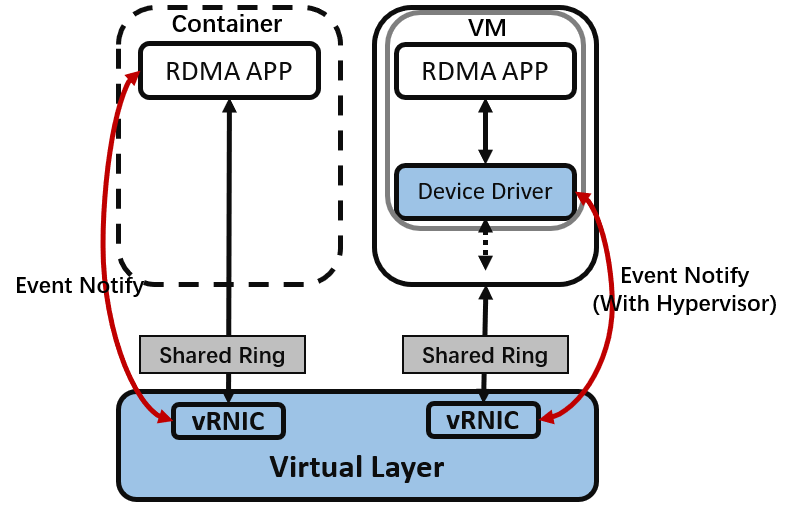
\includegraphics[width=1.0\linewidth]{images/interface-general}
		\caption{Unified vRNIC Driver}
		\label{fig:vrnic-driver}
	\end{figure}
	
The goal of the device driver is to support I/O process inside each guest. As shown in in Figure~\ref{fig:vrnic-driver},  the commands of RDMA application be forwarded into the memory-shared queue, and trigger events to notify the vRNIC to process them; similarly, the device driver receives interrupt notifications and reads the result from vRNIC. In short, the device driver can be implemented by a lightweight kernel module.
	
For generality, As shown in in Figure~\ref{fig:vrnic-driver}, the same design as virtual machines is adopted for containers: in I/O channel, the file-based shared queue is also used; in the synchronization mechanism, the same event notification mechanism is used. But remind the container does not fall into the monitor or inject interrupts during the synchronization.

For multiple containers and virtual machines, if shared memory files for vRNIC driver are not isolated, they can be discovered by every container through scanning files. In order to solve this problem, we run the virtual machine in a isolated container environment. As shown in in Figure~\ref{fig:interface-isolate}, based on the container's mount namespace~\cite{mount-ns}, we respectively place the shared files of each vRNIC in the dedicated directories and mounts each directory to the corresponding container(including containers running virtual machines). As a result, due to the isolation of the mount namespace, the shared files of each vRNIC in the virtualization layer are only visible to the used container or virtual machine.  

\begin{figure}[!ht]
	\centering
	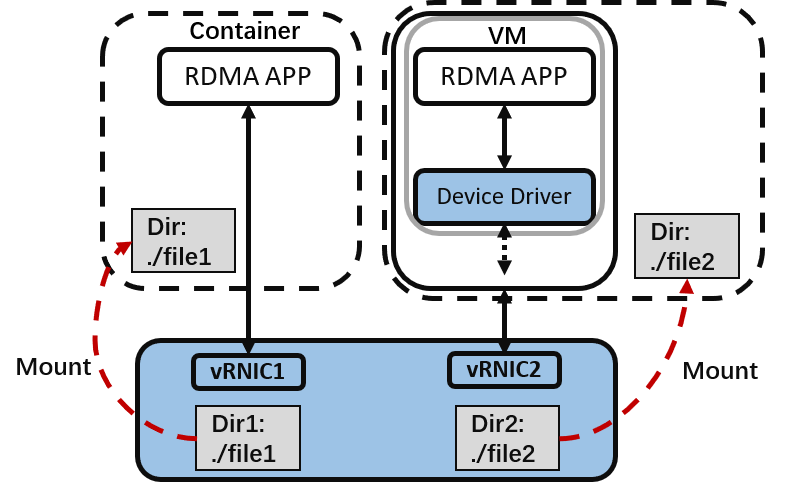
\includegraphics[width=1.0\linewidth]{images/interface-isolate}
	\caption{Isolation for vRNIC driver}
	\label{fig:interface-isolate}
\end{figure}


\subsection{Performance Optimization}

Trough vRNIC driver, all commands of RDMA applications can be excuted in vRNICs. However, in data path of vRNIC, there is still data-copy. Also, the data commands are forwarded to vRNIC for execution. These brings the data-copy or context-switch latency for RDMA applications. 

To address above performance problems, we map RDMA resources between vRNICs and appications. However, there are two different RDMA resources for vRNICs: resources in host physical memory (such as QPs, MRs), resources in physhical RNIC (e.g. DoorBell registers). 

(1) For QPs or MRs: The fact of zero-copy is that both processes have common available physical memory pages. Same as native RDMA, the zero-copy contents are including the RDMA work request in QPs and data in MRs. 
Similar as the above I/O channels, we use shared memory to map applications' memroy to vRNICs' RDMA resources (e.g. QPs and MRs). And this mapping is feasible for both VMs and containers.

\begin{figure}[!ht]
	\centering
	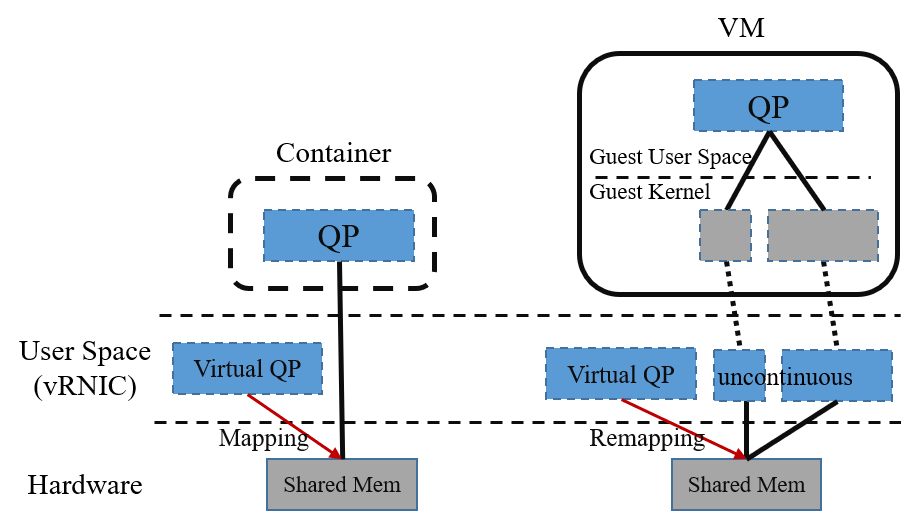
\includegraphics[width=1.0\linewidth]{images/zero-copy}
	\caption{Mapping QP to vRNIC}
	\label{fig:zero-copy}
\end{figure}

However, in the virtual machine, due to the memory management mechanism of guest operating system, the virtual machine's physical memory of the RDMA resource may be not continuous, and the mapped memory area in vRNIC is not continuous like Figure~\ref{fig:zero-copy}. So, vRNIC cannot map the virtual memory area as a virtual RDMA resource to RNIC. To solve this problem, the virtual memory remapping mechanism in user space is used. It remaps the discontinuous RDMA resource virtual memory area in vRNIC to the a block of continuous virtual memory, and the sequence of mapped physical memory page must be unchanged.

(2) For doorbells: Pressing the doorbell is necessary in RDMA data path to drive RNIC. In vRNIC, the doorbell that is mapped to physical RNIC, still need to be mapped to RDMA application to meet bypassing. Otherwise, the pressing command needs be forward to vRNIC and that’s imports apparent latency in data path.

However, the RDMA application and the vRNIC belong to two different processes on the host, and they have isolated virtual address spaces. At the same time, the doorbell register is in the device address space and cannot be mapped by shared memory. The key to solving this problem is that the process of RDMA application needs to know the physical address of the doorbell register.

\begin{figure}[!ht]
	\centering
	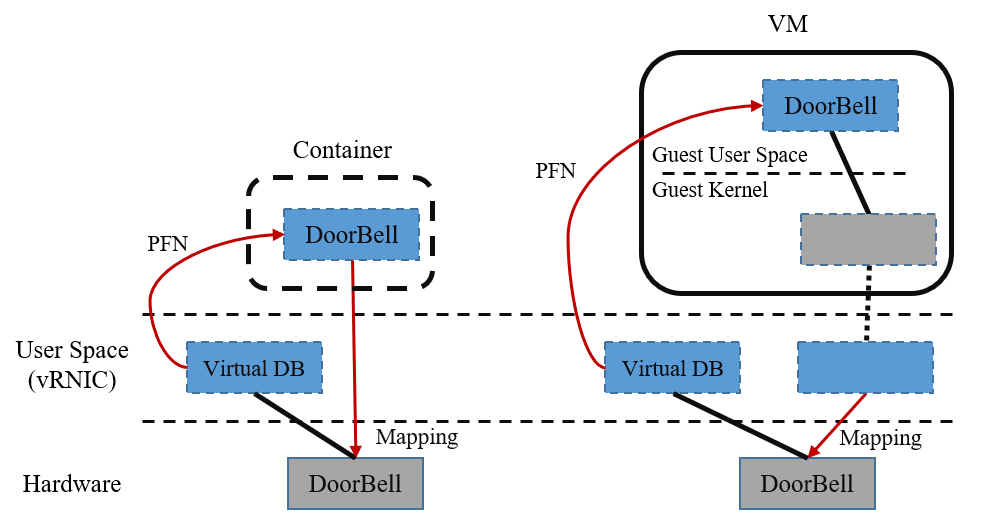
\includegraphics[width=1.0\linewidth]{images/by-pass}
	\caption{Mapping DB from vRNIC}
	\label{fig:by-pass}
\end{figure}

Therefore, when an RDMA application creates a RDMA context, as shown in Figure~\ref{fig:by-pass}, it sends a request to the vRNIC at first. Under the supervision of virtual layer, vRNIC forwarded to application with the corresponding physical address of the doorbell, commonly the physical page number. After that, the application maps its doorbell virtual address to the physical page in its own process, that needs the host kernel and hypervisor if the application in virtual machines.

